% !TeX root = ../../../latex-talk.tex

\section{是什么}

\begin{frame}
  \frametitle{\TeX{}}
  \begin{columns}[c]
    \begin{column}{0.7\textwidth}
      \begin{center}
        \rmfamily\Huge
        \highlight[structure]{\TeX{}}
      \end{center}
      \begin{center}
        \parbox{0.75\textwidth}{
          \TeX{} 是由斯坦福大学教授高德纳
          (Donald E.~Knuth)于 1977 年开始开发的排版引擎。目前仍在更新,最新版本号为 3.141592653 \link{https://tug.org/TUGboat/tb42-1/tb130knuth-tuneup21.pdf}。
        }
      \end{center}
    \end{column}
    \begin{column}{0.3\textwidth}
      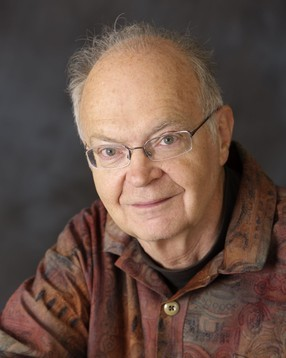
\includegraphics[width=.8\columnwidth]{support/images/Knuth.jpg}
    \end{column}
  \end{columns}
  \note{\emph{这一部分背景介绍大家可以了解一下,暂时跳过。}
  \LaTeX{} 这个词由两个部分组成,\hologo{La} 和 \TeX{}。那我们首先了解一下 \TeX{} 是什么。
  \TeX{} 是由斯坦福大学的教授高德纳于 1977 年开始开发的排版引擎,它已经有三十多年的历史了,
  目前仍在更新,版本号(3.141592653)将会趋近于 $\pi$ 的取值,高德纳最近还在给 \textsl{TUGBoat} 写稿子
  \link{https://tug.org/TUGboat/tb42-1/tb130knuth-tuneup21.pdf},
  关于 \TeX{} 今年又做了哪些改进。}
\end{frame}

\begin{frame}
  \frametitle{\LaTeX{}}
  \begin{columns}[c]
    \begin{column}{0.7\textwidth}
      \begin{center}
        \rmfamily\Huge
        \highlight[structure]{\LaTeX{}}
      \end{center}
      \begin{center}
        \parbox{0.75\textwidth}{
          \LaTeX{} 是最早在 1985 年由现就职于微软的 Leslie Lamport 开发的一种 \TeX{} \textbf{格式}\footnotemark,使用一些列宏和扩展宏包来简化 \TeX{} 的使用。现在由 \LaTeX{} Project 的成员维护。现在广泛使用的版本是 \LaTeXe{},最新的版本为 \LaTeX3(2020 年 10 月后默认内置)。
        }
      \end{center}
    \end{column}
    \begin{column}{0.3\textwidth}
      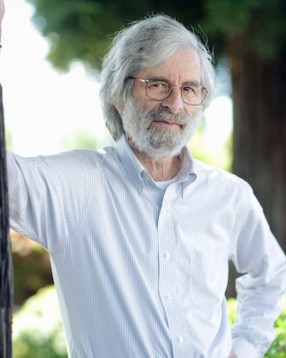
\includegraphics[width=.8\columnwidth]{support/images/Lamport.jpg}
    \end{column}
  \end{columns}
  \footnotetext{\hologo{ConTeXt} 也是一种 \TeX{} 格式 \link{https://www.contextgarden.net/}。}
  \note{\emph{这一部分的背景介绍大家可以了解一下,暂时跳过。}
  \LaTeX{} 是最早由现就职于微软的 Leslie Lamport 开发的一种 \TeX{} 格式(与其对标的是
  \hologo{ConTeXt}\link{https://www.contextgarden.net/}),主要也是为了简化 \TeX{} 的使用。
  现在主要由 \LaTeX{} 开发组维护,现在广泛使用的版本是 \LaTeXe{},最新的版本为 \LaTeX3,
  在 2020 年 10 月后默认内置,所以要尽可能使用较新的发行版,以充分发挥其功能。}
\end{frame}

\begin{frame}
  \frametitle{程序}
  \begin{columns}[c]
    \begin{column}{0.7\textwidth}
      \begin{center}
        \rmfamily\Huge
        \highlight[structure]{\hologo{pdfLaTeX}}
      \end{center}
      \begin{center}
        \parbox{0.7\textwidth}{
          \hologo{pdfLaTeX} 是为了编译一个 \LaTeX{} 文档而运行的程序。实际上底层在运行一个叫 \hologo{pdfTeX} 的引擎,并预装了对应的 \LaTeX{} \textbf{格式}。为了利用临时文件,可能就需要多次运行程序。
        }
      \end{center}
    \end{column}
    \begin{column}{0.3\textwidth}
      \begin{block}{}
        \ttfamily\small
        > \highlight{pdflatex} main.tex\\
        This is pdfTeX, Version 3.141592653-
        2.6-1.40.23 (MiKTeX 21.10)\\
        entering extended mode\\
        \highlight{LaTeX2e} <2021-11-15>\\
        \highlight{L3} programming layer <2021-11-22>
      \end{block}
    \end{column}
  \end{columns}
  \note{\hologo{pdfLaTeX} 是为了编译一个 \LaTeX{} 文档而运行的程序。}
\end{frame}

% \begin{frame}
%   \frametitle{引擎}
%   \begin{columns}[c]
%     \begin{column}{0.7\textwidth}
%       \begin{center}
%         \rmfamily\Huge
%         \highlight[structure!70]{pdf}\hologo{La}\highlight[structure!70]{\TeX{}}
%       \end{center}
%       \begin{center}
%         \parbox{0.7\textwidth}{
%           pdf\TeX{} 是编译 \TeX{} 文档(以 \texttt{.tex} 结尾)的\textbf{引擎}---可以理解 \TeX{} 指令的\textbf{程序}。
%         }
%       \end{center}
%     \end{column}
%     \begin{column}{0.3\textwidth}
%       \begin{block}{}
%         \ttfamily\small
%         > pdflatex main.tex\\
%         This is \highlight[structure!70]{pdfTeX}, Version 3.141592653-
%         2.6-1.40.23 (MiKTeX 21.10)
%         entering extended mode\\
%         LaTeX2e <2021-11-15>\\
%         L3 programming layer <2021-11-22>
%       \end{block}
%     \end{column}
%   \end{columns}
%   \note{实际上底层在运行一个叫 \hologo{pdfTeX} 的引擎,并预装了对应的 \LaTeX{} 格式。}
% \end{frame}

\begin{frame}[label={frame:engine}]
  \frametitle{程序}
  \begin{table}
    \caption{主流 \hologo{(La)TeX} 程序
    \footnote{(u)p\TeX{} 是日语最常用的引擎,生成 \texttt{.dvi},支持 Unicode。}\footnote{Ap\TeX{} \link{https://github.com/clerkma/ptex-ng} 具有底层 CJK 支持,内联 Ruby,Color Emoji。}}
    \footnotesize
    \begin{stampbox}
      \begin{tabular}{c>{\raggedright}*{3}{p{3.5cm}}}
        \alert{引擎}     & \hologo{pdfTeX}   & \hologo{XeTeX}   & \hologo{LuaTeX}   \\
        \alert{程序}     & \hologo{pdfLaTeX} & \hologo{XeLaTeX} & \hologo{LuaLaTeX} \\
        \alert{特点}     & 直接生成 PDF,支持 micro-typography  & 支持 Unicode、OpenType 与复杂文字编排 (CTL) & 支持 Unicode,内联 Lua,支持 OpenType \\
      \end{tabular}
    \end{stampbox}
  \end{table}

  \begin{center}
    \parbox{.9\textwidth}{
      \hologo{pdfLaTeX} 不支持 Unicode。为了排版中文,大部分情况下应当使用 \hologo{XeLaTeX},而 \hologo{LuaLaTeX} 速度相对较慢。\faWindows{} 可以在一些情况下使用 \hologo{pdfLaTeX}。
    }
  \end{center}
  \note{当然为了排版中文,已经不再推荐使用 \hologo{pdfLaTeX} 了,应该使用
  \hologo{XeLaTeX} 或者 \hologo{LuaLaTeX},当然后者的速度还是相对较慢,
  它们支持 Unicode 编码,并可以使用 OpenType 字体的全部功能。
  当然 \faWindows{} 平台下在某些追求速度的情况下,
  还是可以试着使用 \hologo{pdfLaTeX} 的。

  \hologo{LuaLaTeX} 理想情况下不慢,但是使用一些宏包后会破坏理想状态,
  也会因配置产生不同的结果,不同的操作系统在 I/O 速度上的不同也会导致不同的时间。

  \hologo{pdfLaTeX} 也支持,只不过需要先生成 tfm \TeX{} 字体度量文件,后续使用 \TeX{}
  自身的配置方法,只能使用 7 比特或 8 比特字体。}
\end{frame}

% \begin{frame}
%   \paragraph{\hologo{pdfLaTeX}} \TeX{} 和 \LaTeX{} 被广泛使用之前,它们只需内置支持欧洲语言即可。在 Unicode 出现之前,\LaTeX{} 提供了许多种\textbf{文件编码}来允许很多语言的文字以原生的方式输入,\hologo{pdfLaTeX} 也只需要使用 8 位文件编码和 8 位字体。
% \end{frame}

